\documentclass[aap,authoryear, preprint]{imsart}
\RequirePackage[OT1]{fontenc}
\RequirePackage{amsthm,amsmath}
\RequirePackage{natbib}
% \RequirePackage[colorlinks,citecolor=blue,urlcolor=blue]{hyperref}
\usepackage{amsfonts}
\usepackage{amsmath}
\usepackage{amssymb}
\usepackage{amsthm}
\usepackage{array}
\usepackage{bbm}
\usepackage{bm}
\usepackage{booktabs}
\usepackage[makeroom]{cancel}
\usepackage{color}
\usepackage{float}
\usepackage{enumerate}
\usepackage{graphicx}
\usepackage{mathtools}
\usepackage{newfloat}
% \usepackage{subcaption}
\usepackage{tocloft}
\usepackage{wrapfig}
% settings
%\pubyear{2005}
%\volume{0}
%\issue{0}
%\firstpage{1}
%\lastpage{8}
\arxiv{arXiv:0000.0000}

\startlocaldefs
\numberwithin{equation}{section}
\theoremstyle{plain}
\newtheorem{prop}{Proposition}
\endlocaldefs

\begin{document}

\begin{frontmatter}
\title{Dynamic Gene coexpression Analysis with Correlation Modeling}
\runtitle{Dynamic Gene coexpression Analysis}

\begin{aug}
\author{\fnms{Tae} \snm{Kim}\ead[label=e1]{tk382@uchicago.edu}}
\and
\author{\fnms{Dan} \snm{Nicolae}\ead[label=e2]{nicolae@uchicago.edu}}

\affiliation{University of Chicago}
\address{5747 South Ellis Avenue\\
Chicago, IL 60637}
\end{aug}

\begin{abstract}
In many biological studies on the transcriptome, the correlation of genes might fluctuate with quantitative factors such as genetic ancestry. We propose a method that can model the covariance between two variables to vary against a continuous covariate. For the bivariate case, we propose a score test statistic that is computationally simple and robust to model misspecification of the covariance term $\rho$. Subsequently, we expand the method to test relationships between one highly connected gene, such as transcription factors, and several other genes to obtain a more global view of the dynamic of the coexpression network. Simulations show that the proposed method has higher statistical power than the alternatives, works under more diverse scenarios, and is computationally much cheaper. We apply this method to African American subjects from GTEx to analyze the dynamic behavior of their gene coexpression against genetic ancestry, and we identify transcription factors whose coexpressions with their target genes change with the genetic ancestry. We believe this method can be applied to a wide array of problems that require covariance modeling.
\end{abstract}

\begin{keyword}
coexpression; network; heteroskedasticity; score test; GTEx; admixed population
\end{keyword}

\end{frontmatter}
\section{Introduction}
\subsection*{}
Gene coexpression, the covariance structure of gene expression data, shows how genes are functionally connected and provides insights into the design of the transcriptional regulatory system. Ideally, such a complicated biological system can be fully understood through longitudinal observations in multiple and diverse cell types that capture the dynamics of the system. In reality, however, such comprehensive measurements are often unavailable or too expensive, and the expression dynamics must be captured instead through cross-sectional or tissue-specific data sets. In such cases, investigating the dependence structure can be useful. The dependence structure can be especially valuable for characterizing how few key genes are connected to the rest of the transcriptome. For example, we can focus on one transcription factor --- genes that help turn transcription of genes on and off --- and study how it is connected to its target genes. To further investigate this problem, we define ``local connectivity" of a transcription factor as its overall connectivity to its target genes.\\

Consider this biological problem: how does local connectivity vary across various phenotypic conditions?  Past studies have investigated similar problems, such as how subjects in distinct disease groups show distinct coexpression patterns, contributing to a better understanding of disease at a molecular level (\cite{de2010differential}). Here, we focus on understanding how coexpression changes with quantitative traits, not discrete conditions such as disease status, and hence we study the dynamic nature of coexpression. As an example of a quantitative trait, we use genetic ancestry. Ancestry is known to play a critical role in other molecular phenotypes including DNA methylation and gene expressions (\cite{galanter2017differential, price2008effects}), and so we believe it has an important role in gene dynamics and gene networks as well. In this paper, we study how the local connectivity of transcription factor genes changes with ancestry. Specifically, we study the gene coexpression of African American subjects to identify candidate transcription factors whose effects on their targets vary with the proportion of African ancestry in their genome. This analysis will lead to a better comprehension of how genes are differentially regulated in distinct populations. \\

The above biological problem can be investigated using multivariate statistical models of gene expression with a covariance structure (characterizing connectivity) that depends on one or more features (such as ancestry). This paper focuses on testing the contribution of ancestry on the covariance matrix, and we start from its simplest form by studying the expression levels of two genes. We construct a statistical model that can explain how their correlation varies against genetic ancestry and use that to test if the correlation is constant across conditions. We generalize it to the local connectivity of a transcription factor by meta-analyzing the pairwise statistics. Note that covariance modeling for multivariate data is important in many applications outside the field of genetics. Variance modeling has been widely studied in the context of heteroskedasticity (\cite{breusch1979simple, glejser1969new, white1980heteroskedasticity}), and correlation modeling under discrete conditions has been studied in the context of the differential network (\cite{ideker2012differential}), but dynamic correlation modeling has been less explored. \\

\cite{li2002genome} and \cite{li2004system} addresses the most similar scientific problem to ours, using the term ``liquid association" (LA) to conceptualize the internal evolution of the coexpression pattern for a pair of genes. They analyze the coexpression that changes across different unobserved cellular states that are represented by the expression level of another gene as a proxy. Other studies have built on the liquid association to better identify cell states that affect coexpression (\cite{yan2017detecting, yu2018new}), most focusing on expanding the test to genome-scale. However, methods based on liquid association have some limitations. First, it restricts the covariate to be a 1-dimensional vector, and cannot be generalized to more realistic scenarios. Second, it treats the covariate as a random variable that follows a normal distribution, which genetic ancestry does not, so it cannot be used for our application. Third, it only tests the linear relationship between the covariate and the coexpression. Lastly, the corresponding test statistic does not have a closed-form null distribution and requires a permutation test, leading to computational inefficiency. \\

We propose a methodology for the continuously-varying covariance problem. We transform the likelihood function of bivariate normal variables to effectively change the multivariate covariance modeling problem to a univariate variance modeling problem. We then apply a traditional score test for heteroskedasticity (\cite{breusch1979simple}) where the null hypothesis is that the coexpression does not vary with the covariate. This method is generalizable to non-normal, multivariate covariates, and it is also applicable to a non-linear relationship between the variance and the covariate. Moreover, the score test statistic asymptotically follows a chi-squared distribution, and hence it is easily expandable to a large number of tests without excessive computational burden. Subsequently, we tackle the local connectivity problem by expanding the scope of the problem from the relationship of two genes to the relationships between one gene and multiple genes by combining the test statistics. When the number of genes in the local cluster is smaller than the sample size, the desired statistical properties apply to the new combined test statistic as well. \\

The rest of the paper is organized as follows. First, we lay out the framework for the score test that investigates whether the covariance between bivariate normal variables varies against a continuous covariate $X$. Then we propose a way to combine the pair-wise test statistics for one gene and test the global null that the local connectivity of one variable does not change with genetic ancestry. In the simulation section, we show that the proposed method has distinct advantages compared to alternatives such as the likelihood ratio test or liquid association. Finally, we share our real data analysis results using Gene-Tissue Expression (GTEx) data for African Americans' transcriptome and genome. We end with a discussion about limitations of the method, possible future directions, and potential applications to fields outside genetics.

\section{Methods}
\subsection{Test for connectivity between two genes \label{sec:framework2}}
Consider 2-dimensional data for $N$ subjects $\bm{y}_i \in \mathbb{R}^2$, $i = 1, 2, \cdots, N$ independently following the bivariate normal distribution. There are two covariate matrices $Z \in \mathbb{R}^{N \times R}$ and $X \in \mathbb{R}^{N \times P}$, each for the mean term and the variance term, respectively. They are both assumed to be full rank. We notate each element of $X$ and $Z$ as $\{x_{ip}\}_{i=1,p=1}^{N,P}$ and $\{z_{ir}\}_{i=1,r=1}^{N,R}$.
\begin{equation}
\begin{multlined}
    \begin{bmatrix} y_{i1} \\ y_{i2} \end{bmatrix} = 
    \begin{bmatrix} b_{1} \\ b_{2} \end{bmatrix} + 
    \begin{bmatrix} \bm{z}_i^T \bm{\beta}_1 \\ \bm{z}_i^T \bm{\beta}_2 \end{bmatrix} + 
    \begin{bmatrix} {u_{i1}} \\ {u_{i2}} \end{bmatrix}\\
    \begin{bmatrix} {u_{i1}} \\ u_{i2} \end{bmatrix} 
    \sim \mathcal{N}\left(
        \begin{bmatrix} 0 \\ 0 \end{bmatrix}, 
        \begin{bmatrix} \rho_{11} & \rho_{12}(\bm{x}_i) \\ 
        \rho_{12}(\bm{x}_i) & \rho_{22} \end{bmatrix}
    \right)
    \end{multlined}
    \label{eq:framework_2genes}
\end{equation}
$\bm{\beta}_1$ and $\bm{\beta}_2$ are coefficients with length $R$  for the mean term $Z$. $\rho_{11}$ and $\rho_{22}$ are fixed scalars but $\rho_{12}$ varies with the covariate. We define $\bm{\alpha} \in \mathbb{R}^{P}$ and a scalar $\alpha_0$ as the linear coefficients to model $\rho_{12}$ as follows.
\begin{equation}
    \rho_{12}(\bm{x}_i) = \rho_{12}(\bm{x}_i^T\bm{\alpha} + \alpha_0) \label{eq:rho}
\end{equation}
Our parameter of interest is $\bm{\alpha}$ while all others --- $\alpha_0$, $\bm{b}$, $\bm{\beta}$, $\rho_{11}$, $\rho_{22}$ --- are nuisance parameters. Our goal is to develop a method that tests the following null hypothesis
\begin{equation}
    H_0: \bm{\alpha} = \bm{0}.
    \label{eq:null}
\end{equation}
Under the null hypothesis, $\rho_{12}(\bm{x}_i, \bm{\alpha}) = \rho_{12}(\alpha_0)$ is a constant. The linearity and additivity assumptions in (\ref{eq:rho}) are standard, and since $\rho_{12}$ can take any non-linear form, (\ref{eq:rho}) still is a flexible framework. Before we introduce the detailed methodology, we first present our result below.

\begin{prop}
Consider the model in (\ref{eq:framework_2genes}). If all the covariates $X$ are centered, $\sum_{i=1}^{N} x_{ip} = 0$ for $p = 1, \cdots, P$, and the non-diagonal term follows the function $\rho_{12}$ as defined in (\ref{eq:rho}), the score statistic does not depend on the unknown function $\rho_{12}$ and follows $\chi_P^2$ under the null hypothesis (\ref{eq:null}). 
\label{theorem:q}
\end{prop}

The score statistic is later introduced in (\ref{eq:q}). The model (\ref{eq:framework_2genes}) is close to a multivariate regression model of $\bm{y}_i$ against the mean term $\bm{z}_i$ with intercept $\bm{b}_0$, slope $\begin{bmatrix} \bm{\beta}_1 & \bm{\beta}_2 \end{bmatrix}$, and error term $\bm{u}_i$. The difference is that its error variance depends on the covariate $\bm{x}_i$. The function $\rho_{12}$ represents an unknown form of heteroskedasticity between the two variables $1$ and $2$. In the context of gene coexpression of African Americans, $\bm{y}_i$ is gene expression level of an African American individual $i$ at two selected genes, and $\bm{x}_i$ is a $P$-dimensional covariate matrix for individual $i$ that holds information about genetic ancestry. It can be a scalar that represents the proportion of African ancestry in the genome, a vector of the first few principal components of the genotypes, or a vector of local ancestry at multiple loci. In the application example in section \ref{sec:applications}, we focus on scalar $\bm{x}_i$ for straightforward interpretability. \\

With some mathematical tweaks, we can write the likelihood of (\ref{eq:framework_2genes}) as follows
\begin{equation}
\begin{multlined}
\ell(\bm{\alpha}, \bm{b}, \bm{\beta}, \rho_{11}, \rho_{22}) = \\
-\frac{N}{2} log(2\pi) - \frac{1}{2} \sum_{i=1}^{N} log (\sigma_{wi}^2) - \sum_{i=1}^{N} \frac{(w_i - \mu_{wi})^2}{2\sigma_{wi}^2}\\
-\frac{N}{2} log(2\pi) - \frac{1}{2} \sum_{i=1}^{N} log (\sigma_{vi}^2) - \sum_{i=1}^{N} \frac{(v_i - \mu_{vi})^2}{2\sigma_{vi}^2}\\
= -Nlog(2\pi) - \frac{1}{2} \sum_{i=1}^{N}log(\sigma_{wi}^2) - - \frac{1}{2} \sum_{i=1}^{N} log(\sigma_{vi}^2) - \sum_{i=1}^{N} \frac{u_{wi}^2}{2\sigma_{wi}^2} - \sum_{i=1}^{N} \frac{u_{vi}^2}{2\sigma_{vi}^2}
\end{multlined}
    \label{eq:likelihood_2genes}
\end{equation}
with the variables defined as following.
\begin{align*}
w_i = \frac{y_{i1}}{\sqrt{\rho_{11}}} + \frac{y_{i2}}{\sqrt{\rho_{22}}}, 
\hspace{6mm} &
v_i = \frac{y_{i1}}{\sqrt{\rho_{11}}} - \frac{y_{i2}}{\sqrt{\rho_{22}}},\\
u_{wi} = \frac{u_{i1}}{\sqrt{\rho_{11}}} + \frac{u_{i2}}{\sqrt{\rho_{22}}}, 
\hspace{6mm} &
u_{vi} = \frac{u_{i1}}{\sqrt{\rho_{11}}} - \frac{u_{i2}}{\sqrt{\rho_{22}}}.\\
\sigma_{wi}^2 = 2 + \frac{2\rho_{12}(\bm{x}_i^T \bm{\alpha})}{\sqrt{\rho_{11}\rho_{22}}}, \hspace{6mm}&
\sigma_{vi}^2 = 2 - \frac{2\rho_{12}(\bm{x}_i^T \bm{\alpha})}{\sqrt{\rho_{11}\rho_{22}}},\\
\mu_{wi} = \frac{{b}_1}{\sqrt{\rho_{11}}} + \frac{{b}_2}{\sqrt{\rho_{22}}} + &\bm{z}_i^T \left(\frac{\bm{\beta}_1}{\sqrt{\rho_{11}}} + \frac{\bm{\beta}_2}{\sqrt{\rho_{22}}}\right),\\
\mu_{vi} = \frac{{b}_1}{\sqrt{\rho_{11}}} - \frac{{b}_2}{\sqrt{\rho_{22}}} + &\bm{z}_i^T \left(\frac{\bm{\beta}_1}{\sqrt{\rho_{11}}} - \frac{\bm{\beta}_2}{\sqrt{\rho_{22}}}\right)
\end{align*}
The intuition of (\ref{eq:likelihood_2genes}) is to think of $w_i$ and $v_i$ as the normalized sum and difference of the two variables. This way, the likelihood is expressed as the product of two independent univariate likelihood instead of the more complicated bivariate likelihood. Now the covariance problem is effectively transformed to modeling the variance problem, and we can apply the results from literature on univariate heteroskedasticity. Given the likelihood (\ref{eq:likelihood_2genes}), we have two well-known tools to test the null hypothesis (\ref{eq:null}): likelihood ratio test and Rao's score test (\cite{breusch1979simple}). \\

The likelihood ratio test has a few disadvantages compared to the score test. It requires the full specification of the function $\rho$ to estimate the maximum likelihood estimate (MLE) of $\bm{\alpha}$ both under the null hypothesis and under the alternative hypothesis. Possible functions of $\rho_{12}$ are any kind of sigmoid function bound to $(-\sqrt{\rho_{11}\rho_{22}}$, $\sqrt{\rho_{11}\rho_{22}})$ such as logistic function, hyperbolic tangent function, or any cumulative distribution supported on the whole real line. This modeling strategy leads to one disadvantage; as mentioned in the previous section, we would like to impose as few assumptions on the specific form of heteroskedasticity as possible. If $\rho_{12}$ is highly misspecified, we sacrifice the statistical power. Another disadvantage is that most of the reasonable assumptions of $\rho$, such as the sigmoid functions mentioned above, do not lead to a closed form MLE of $\bm{\alpha}$ under the alternative hypothesis. It would require us to numerically optimize the likelihood, leading to computational inefficiency, especially when the test space is large as in our application of gene coexpression. \\

On the other hand, Rao's score test, unlike the likelihood ratio test, only requires the MLE of $\bm{\alpha}$ under the null hypothesis (\cite{rao1973linear}). Moreover, under our linear and additive model ($\rho_{12}(\bm{x}_i) = \rho_{12}(\bm{x}_i^T\bm{\alpha})$), the test statistic does not depend on the form of $\rho_{12}$ while maintaining its asymptotic property as long as $\rho_{12}$ is twice differentiable. In order to test (\ref{eq:null}), we expand the result from \cite{breusch1979simple} to derive the test statistic.\\ 

The score test allows us to replace all the nuisance parameters with the MLEs under the null hypothesis. We can therefore replace $\alpha_0, \bm{\beta}$, $\bm{b}$, $\rho_{11}$, and $\rho_{22}$ with their respective MLEs that result from ordinary least squares linear regression. The first derivative of the likelihood evaluated at $\bm{\alpha}=\bm{0}, \alpha_0 = \hat{\alpha}_0, \bm{\beta} = \bm{\hat{\beta}}$, $\bm{b} = \bm{\hat{b}}$, $\rho_{11} = \hat{\rho}_{11}$, and $\rho_{22} = \hat{\rho}_{22}$ is as follows. We also define $\hat{u}_{i1}$ and $\hat{u}_{i2}$ as the OLS residuals from (\ref{eq:framework_2genes}).
\begin{equation}
\begin{multlined}
\bm{\tilde{d}}_{\alpha} = \frac{\partial \ell(\bm{\alpha}, \bm{b}_0, \bm{\beta})} {\partial \bm{\alpha}}\mid_{\bm{\alpha}=\bm{0}, \alpha_0 = \hat{\alpha}_0, \bm{\beta} = \bm{\hat{\beta}}, \bm{b} = \bm{\hat{b}}, \rho_{11} = \hat{\rho}_{11}, \rho_{22} = \hat{\rho}_{22}} =\\
-\frac{\rho_{12}'(\alpha_0)}{2\sqrt{\rho_{11}\rho_{22}}} \sum_{i=1}^{N} \left(
    \frac{\bm{x}_i}{\hat{\sigma}_{w}^2} 
    \left( 1-\frac{\hat{u}_{wi}^2}{\hat{\sigma}_{w}^2}\right) - 
    \frac{\bm{x}_i}{\hat{\sigma}_{v}^2} 
    \left( 1-\frac{\hat{u}_{vi}^2}{\hat{\sigma}_{v}^2}\right) 
    \right)
\end{multlined}
\label{first_derivative}
\end{equation}
where the error variance estimates are $\hat{\sigma}_w^2 = \sum_{i=1}^{N} \hat{u}_{wi}^2/N$ and $\hat{\sigma}_{vi}^2 = \sum_{i=1}^{N}\hat{u}_v^2/N$. The derivation is in the appendix. The Fisher information for $\bm{\alpha}$ is
\begin{equation}
\begin{multlined}
        \tilde{\mathcal{I}}_{\bm{\alpha}\bm{\alpha}^T} = \mathcal{I}_{\bm{\alpha}\bm{\alpha}^T}\mid_{
        \bm{\alpha}=\bm{0}, 
        \alpha_0 = \hat{\alpha}_0,
        \bm{b} = \bm{\hat{b}},
        \bm{\beta} = \bm{\hat{\beta}},
        {\rho}_{11} = \hat{\rho}_{11},
        {\rho}_{22} = \hat{\rho}_{22}}\\
        = \frac{{\rho'}^2_{12}(\hat{\alpha}_0)}{4\hat{\rho}_{11}\hat{\rho}_{22}}\cdot 2 \cdot \left(\frac{1}{\hat{\sigma}_{w}^2} +  \frac{1}{\hat{\sigma}_{v}^2}\right) \sum_{i=1}^{N} \bm{x}_i \bm{x}_i^T
    \end{multlined}
\end{equation}
All other second-order derivatives --- 
$\tilde{\mathcal{I}}_{\bm{\alpha}\bm{\beta}^T}$,
$\tilde{\mathcal{I}}_{\bm{\alpha}\alpha_0}$,
$\tilde{\mathcal{I}}_{\bm{\alpha}\rho_{11}}$,
$\tilde{\mathcal{I}}_{\bm{\alpha}\rho_{22}}$,
$\tilde{\mathcal{I}}_{\bm{\alpha}\bm{b}^T}$ --- are $\bm{0}$ when the covariates are centered. The test statistic $q$ for the variables 1 and 2 is
\begin{equation}
    \begin{multlined}
    q = \tilde{d}_{\bm{\alpha}}^T \tilde{I}_{\bm{\alpha}\bm{\alpha}^T}^{-1}
    \tilde{d}_{\bm{\alpha}}
    =\frac{1}{2}\left( \frac{1}{\hat{\sigma}_w^4}+\frac{1}{\hat{\sigma}_v^4}\right)^{-1}
\left(\sum_{i=1}^{N} \bm{x}_{i} 
\left(
\frac{\hat{\sigma}_w^2-\hat{u}_{wi}^2}{\hat{\sigma}_w^4}- \frac{\hat{\sigma}_v^2-\hat{u}_{vi}^2}{\hat{\sigma}_v^4}
\right)
\right)^T \\
\left( \sum_{i=1}^{N} \bm{x}_i^T \bm{x}_i \right)^{-1}
\left(
\sum_{i=1}^{N} \bm{x}_{i} 
\left(
\frac{\hat{\sigma}_w^2-\hat{u}_{wi}^2}{\hat{\sigma}_w^4}- \frac{\hat{\sigma}_v^2-\hat{u}_{vi}^2}{\hat{\sigma}_v^4}
\right)
\right)
    \end{multlined}
    \label{eq:q}
\end{equation}
where the unknown function $\rho_{12}$ has been canceled out. Every component of the test statistic is easily acquired from the data, and the computational burden is low. Just as importantly, it is flexible as it allows any form of heteroskedasticity $\rho_{12}$. Under this setting, $q$ asymptotically follows $\chi_{P}^2$ (\cite{breusch1979simple}).\\

However, even though the introduced test statistic has convenient asymptotic properties, the inference might not be correct under finite sample size. The error is in the order of $N^{-1}$ (\cite{harris1985asymptotic}), and many Monte Carlo experiments show that the test rejects the null hypothesis less frequently than indicated by its nominal size (\cite{ godfrey1978testing, griffiths1986monte}. In response, corrections have been suggested (\cite{cribari2001monotonic, harris1985asymptotic}), and we apply the method from \cite{honda1988size} to ensure the validity of the asymptotic properties even under the small sample size. The details of the small-sample correction, as well as the detailed derivation of the test statistic, are shown in the Appendix.\\


\subsection{Test for Local Connectivity \label{sec:frameworkK}} 
In section (\ref{sec:framework2}), we proposed the statistic $q$ to test a pair of variables 1 and 2 to measure the evidence that their correlation changes with the covariate $X$. As a natural extension to the pair-wise test statistic, we can repeat the procedure for more than 2 variables. In particular, we can study one transcription factor with  multiple target genes to test whether the local connectivity of the transcription factor varies with genetic ancestry. In this section, we propose a way to combine the test statistics to test a new global null hypothesis. The global null hypothesis for variable $1$ extends (\ref{eq:null}) as follows,
\begin{equation}
    \bm{H}_0^{(1)}: \bm{\alpha}_{12} = \bm{\alpha}_{13} = \cdots = \bm{\alpha}_{1K} = \bm{0},
\label{eq:globalnull}
\end{equation}
where the superscript in $\bm{H}_0^{(1)}$ indicates that the null hypothesis applies to variable 1. Under $\bm{H}_0^{(1)}$, no other variables' correlation with variable 1 changes across the different values of  $X$. We believe testing the global null (\ref{eq:globalnull}) improves the statistical power when the ``hot spot" variables or ``hub" variables are connected to a lot of other nodes forming cliques or modules. In the context of gene coexpression network, we know that transcription factors regulate the gene expression of multiple genes, and if one transcription factor varies with respect to the covariate, the transcriptions of its regulated genes are likely to be correlated with the covariate as well. \\

We propose a way to combine the test statistics to test (\ref{eq:globalnull}). \cite{chen2012exponential} discusses two ways to construct the alternative hypothesis for testing the global null. One way, called a sparse alternative, is to test whether only a small number among all tests have non-zero effects while all other tests are null. Another way is to test if at least one test has a non-zero effect size. Based on our prior knowledge in biology and coexpression network, we assume that there are many small signals instead of few big ones, so we choose the latter. We propose a simple linear combination of the test statistics
\begin{equation}
d_1 = {q}_{12} + {q}_{13} + \cdots + {q}_{1K} = \sum_{k=2}^{K} {q}_{1k}.
\label{eq:d}
\end{equation}
Note that $q$ has been constructed from normalized data of $w$ and $v$ in (\ref{eq:likelihood_2genes}). It is, therefore, the most natural to add them without additional weighting. We believe the statistic $d_1$ in  (\ref{eq:d}) improves the statistical power because even if the effect sizes for each gene pair may be too small to be detected, when combined, they can form a stronger signal. \\

We derive the null distribution of $d_1$ to test (\ref{eq:globalnull}). Although each ${q}_{1k}$ follows $\chi_{P}^2$, they are correlated to one another, so the null distribution is not trivial. We devise a way to simulate the null distribution as a finite sum of Gamma distributions so that we can estimate the empirical quantile of $d_1$. We therefore propose the following.

\begin{prop}
Under the setting of Proposition \ref{theorem:q}, and two additional assumptions that (1) the covariates have been orthogonalized so that 
$\frac{1}{N} \sum_{i=1}^{N} \bm{x}_i \bm{x}_i^T$ is a $P$ by $P$ identity matrix and that (2) none of the variables $y_1, \cdots, y_K$ are perfectly correlated, $d_1$ asymptotically follows the finite sum of Gamma distributions as defined in (\ref{eq:d_dist}) under the global null hypothesis (\ref{eq:globalnull}). 
\end{prop}

To derive the empirical null distribution of $d_1$, We start by re-writing the pairwise score statistic $q$ (omitting gene pair index for now) as a sum of $\chi_1^2$ variables as below. Our null hypothesis tests for all covariates at the same time, so we can orthogonalize $X$ to make $\frac{1}{N} \sum_{i=1}^{N} \bm{x}_i \bm{x}_i^T$ an identity matrix without affecting the testing procedure. Let $\tilde{X}$ be the orthogonalized covariate matrix, and $\tilde{x}_{ip}$ be the corresponding entries with $\sum_{i=1}^{N}\tilde{x}_{ip} = 0$ and $\sum_{i=1}^{N} \tilde{x}_{ip}^2  = n$. Then (\ref{eq:q}) can be alternatively written as follows, where we define $r_{p}.$
\begin{align}
q = \sum_{p=1}^{P}
 \left(\frac{1}{\sqrt{N}}
 \sqrt{\frac{\hat{\sigma}_w^4 \hat{\sigma}_v^4}{\hat{\sigma}_w^4 + \hat{\sigma}_v^4}}
 \sum_{i=1}^{N} x_{ip} \left( \frac{\hat{\sigma}_w^2 - \hat{u}_{wi}^2}{\hat{\sigma}_w^4}
 - \frac{\hat{\sigma}_v^2 - \hat{u}_{vi}^2}{\hat{\sigma}_v^4}
 \right)
\right)^2 = \sum_{p=1}^{P}r_p^2
\label{eq:r}
\end{align}
For each $p$, $r_p$ asymptotically follows the standard normal distribution by the central limit theorem. \\

Now, we acquire a closed-form covariance structure of $r$. First, we begin with a multivariate central limit theorem to write the following in terms of $r$.
\begin{equation}
\bm{r}_{1,p} = \begin{bmatrix}
r_{12,p} \\ r_{13, p} \\ \cdots \\ r_{1K,p}
\end{bmatrix}  \rightarrow N_{K-1}(\bm{0}, H_1) \hspace{5mm} \forall p = 1, \cdots, P
\label{eq:H}
\end{equation}
$H_1$ is a $(K-1) \times (K-1)$ matrix where $(k-1, \ell-1)$th element is $\eta_{1k, 1\ell}$ for $k, \ell = 2, \cdots K$. From (\ref{eq:r}), it is easy to see that $H_1$ has 1 at the diagonals. Also, $\eta_{1k, 1\ell}$ converges in probability to
\begin{equation} \begin{multlined}
\frac{(\tau_{23}+2\tau_{12}\tau_{23})(\tau_{12}^2+1)(\tau_{13}^2+1) + \tau_{12}\tau_{13}(6+2(\tau_{12}^2+\tau_{13}^2+\tau_{23}^2))}{(1-{\tau}_{12}^2)(1-{\tau}_{13}^2)\sqrt{(1+{\tau}_{12}^2)(1+{\tau}_{13}^2)}} \\
- \frac{\tau_{12}(\tau_{13}^2+1)(4\tau_{13}+2\tau_{12}\tau_{23}) + \tau_{13}(\tau_{12}^2+1)(4\tau_{12}+2\tau_{13}\tau_{23})}{(1-{\tau}_{12}^2)(1-{\tau}_{13}^2)\sqrt{(1+{\tau}_{12}^2)(1+{\tau}_{13}^2)}}
% + \frac{3\tau_{12}^3\tau_{13}^3 + \tau_{12}^3\tau_{13} + \tau_{12}\tau_{13}^3 - 5\tau_{12}\tau_{13}}{(1-{\tau}_{12}^2)(1-{\tau}_{13}^2)\sqrt{(1+{\tau}_{12}^2)(1+{\tau}_{13}^2)}}
\label{eq:eta}
\end{multlined} \end{equation}
where 
$${\tau}_{k\ell}= \frac{\rho_{k\ell}}{\sqrt{{\rho}_{kk}{\rho}_{\ell\ell}}}. $$
The derivation is in the Appendix. \\

Note that $d_1$ can be written as the sum of L2 norm of $\bm{r}_{1,p}$ with a known distribution, 
\begin{equation}
d_1 = \sum_{p=1}^{P} \|\bm{r}_{1,p}\|_2^2 = \sum_{p=1}^{P} \sum_{k=2}^K r_{1k,p}^2.
\label{eq:d2}
\end{equation}
Let $H_1 = U_1 \Lambda_1 U_1^T$ be the eigen-decomposition of the covariance matrix $H_1$ in (\ref{eq:H}), where the diagonal matrix $\Lambda$ has eigenvalues $\lambda_{12}, \cdots, \lambda_{1K}$ in a decreasing order. Then, we can next consider the transformation $\bm{r}_{1,p}^* = U\bm{r}_{1,p}$ that follows normal distribution with diagonal covariance matrix $\Lambda_1$. Note that $\|\bm{r}_{1,p}\|_2^2 = \|U\bm{r}_{1,p}\|_2^2$ due to the orthogonal invariance of L2 norm. Then,
\begin{equation}
    \begin{multlined}
    \sum_{p=1}^{P} {r_{1k,p}^*}^2 \sim \Gamma \left( \frac{P}{2}, \frac{\lambda_{1k}}{2} \right), \hspace{5mm} k = 2, \cdots, K\\
    d_1 =  \sum_{p=1}^{P} {r_{12,p}^*}^2 + \cdots +\sum_{p=1}^P{r_{1K,p}^*}^2 \sim \sum_{k=2}^{K} \Gamma \left( \frac{P}{2}, \frac{\lambda_{1k}}{2}\right)
    \end{multlined}
    \label{eq:d_dist}
\end{equation}

Assuming that we know the true, symmetric, positive definite $H_1$, we can acquire positive $\lambda_{1k}$ for $k = 2, \cdots, K$, and we have expressed the null distribution of $d_1$ as the sum of distributions of independent gamma variables. We can computationally simulate this null distribution easily. Alternatively, Moschopoulos (1985) provides another interpretation by expressing the cumulative distribution in a form of infinite sum, but the method is inconvenient in practice.\\

In (\ref{eq:eta}), we define the element-wise mapping $\phi: \Sigma \rightarrow H$. Although we do not know true $\Sigma$ in practice, we can use its maximum likelihood estimate instead as we do with other nuisance parameters. We can see from the construction of $H$ that a well-conditioned, symmetric, positive definite estimate of $\hat{\Sigma}$ leads to a symmetric and positive-definite $\phi(\hat{\Sigma})$ as well. When $N$ is sufficiently larger than $K$, empirical covariance matrix $\hat{\Sigma}$ of $\begin{bmatrix} y_{1i} & y_{2i} & y_{3i} \end{bmatrix}$ is a consistent estimator for $\Sigma$, and replacing $\Sigma$ with $\hat{\Sigma}$ in computing $H$ can guarantee that the test statistic in (\ref{eq:d}) converges in distribution to (\ref{eq:d_dist}). \\

However, when $K$ is larger than $n$, an accurate estimation of $\Sigma$ is a difficult problem. We therefore turn to a permutation test and shuffle the covariate $X$ to test against the true response data that preserves the correlation structure of the network while maintaining the dependence structure of $Y$. The permutation procedure is valid under the assumptions in (\ref{eq:framework_2genes}). \\

We use the sequential precision-improvement permutation test, similar to one suggested by \cite{chen2012exponential}. Permutation test often results in a limited resolution of $p$-values which can lead to imprecise inference especially when we need to correct for the testing of multiple hypotheses. Meanwhile, performing a large number of permutations for every can be computationally wasteful. To find balance, we terminate the permutation procedure if the signal is not strong enough. \\

The detailed procedure is as follows. For every permutation $b = 1, \cdots, B$, we permute the rows (samples) of the covariate matrix $X$ to create $X_b$. Then we compute $d_{kb}$ using $X_b$ and the data matrix $Y$. Then, $d_{kb}$ should follow the null distribution, and the $p$-value for $d_k$ should be computed as a quantile of $d_k$ compared to the empirical distribution of $d_{kb}$ for each $b$. After the minimum number of permutations pre-defined by the user (1000 in our case), we count the number of permutations where $d_{kb}$ is larger than $d_k$. If there are two or more such cases, we terminate the permutation procedure early. Most genes fall into this category leading to $p$-value greater than 0.002. If there are less than 5 such cases observed, we iteratively perform 100 more permutations and re-check the number of $d_{kb}$ with values larger than $d_k$. We repeat until the number of permutations $B$ reaches the predefined maximum number of permutation ($10^5$ in our case), which is designed to give a good enough resolution of $p$-value given the number of tests that we are performing.

\section{Simulation Studies} \label{simulations}
Here, we evaluate the proposed method through simulations. We focus on the pairwise analysis and compare the performance of the proposed score test with two other alternatives - liquid association and the likelihood ratio test. \\

First, we check the calibration of test statistics under the null hypothesis. We sample $X$ from the univariate standard normal distribution to match the required setting of liquid association. We simulate the data matrix $Y$ from 
$$\bm{y}_i \sim \mathcal{N}_2\left(\bm{b}_0 + \bm{z}_i^T\bm{\beta}, \begin{bmatrix} 1 & \bar{\rho} \\ \bar{\rho} & 1 \end{bmatrix}  \right)$$ 
where $\bar{\rho}$ was randomly selected from uniform distribution ranging from -1 and 1 and each element of $\bm{b}_0$ and $\bm{\beta}$ from standard normal distribution. We use $\bm{z}_i = \bm{x}_i$. We test different sample sizes of $N = 500, 100, 30$ to check the behavior of each method under the null hypothesis. For each $N$, we sample $X$ once, and generate $Y$ 1,000 times. The likelihood ratio test was designed to assume hyperbolic tangent model for $\rho$,
\begin{align}
    \rho(\bm{x}_i^T\bm{\alpha}) = \frac{e^{\bm{x}_i^T\bm{\alpha}}-1}{e^{\bm{x}_i^T\bm{\alpha}}+1},
    \label{eq:data_generating_fisher}
\end{align}
which is the inverse of Fisher transformation, 
$\frac{1}{2} \bm{x}_i^T\bm{\alpha} = \frac{1}{2}log \left(\frac{1+\rho}{1-\rho}\right)$. Fisher-transformed $\rho$ asymptotically follows normal distribution, so it works well when $X$ is drawn from normal distribution. We use \textit{optim} function in R to find $\hat{\bm{\alpha}}_{\text{MLE}}$ under the alternative hypothesis. \\

The results show that all three methods control the type I error at the nominal size well, where score and likelihood ratio test statistics both follow $\chi_1^2$ closely. \\

Next we generate the data under the alternative hypothesis to compare the statistical power. So we focus on the case of $N=70$ to reflect the sample size of GTEx data. We again draw $X$ from standard normal distribution. Then, for $i = 1, \cdots, N$, we generate $\rho(\bm{x}_i^T\bm{\alpha})$ from hyperbolic tangent function in (\ref{eq:data_generating_fisher}). Given $\rho$, we draw $Y$ from (\ref{eq:framework_2genes}) with varying levels of $\alpha$, 1000 times each. The hyperbolic tangent model places the likelihood ratio test at an advantage because the model is correctly specified, so as a contrasting case, we use a quadratic model to generate $\rho$ as follows,

\begin{align}
    \rho(\bm{x}_i^T\bm{\alpha}) = (\bm{x}_i^T\bm{\alpha} - 0.1)^2 - 0.99,
    \label{eq:data_generating2_quadratic}
\end{align}

\noindent where subtracting 0.99 is to ensure numerical stability. Since the likelihood ratio test assumes a wrong model, it is expected to lose power. Also, since quadratic function is highly non-linear, liquid association is expected to have poor performance as well. Figure \ref{fig:sim} (a) and (b) show the shape of $\rho$ with respect to $X$ with varying levels of $\alpha$. \\
\begin{figure}
         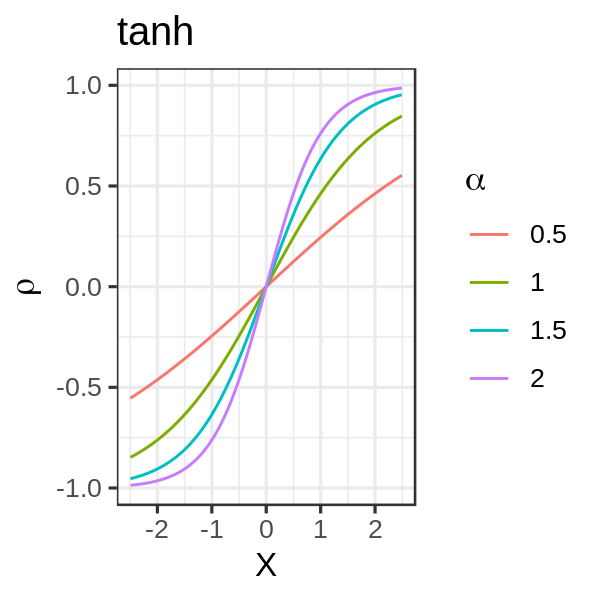
\includegraphics[width=0.32\textwidth]{figures/tanh.png}
         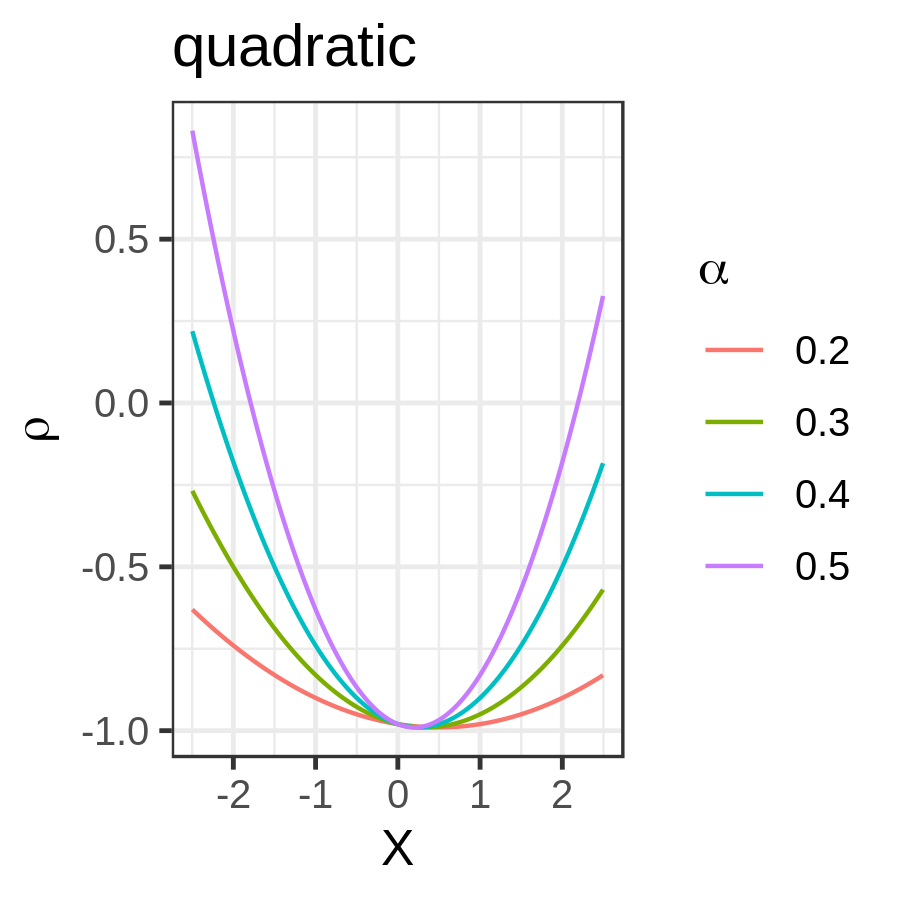
\includegraphics[width=0.32\textwidth]{figures/quadratic.png}
        %  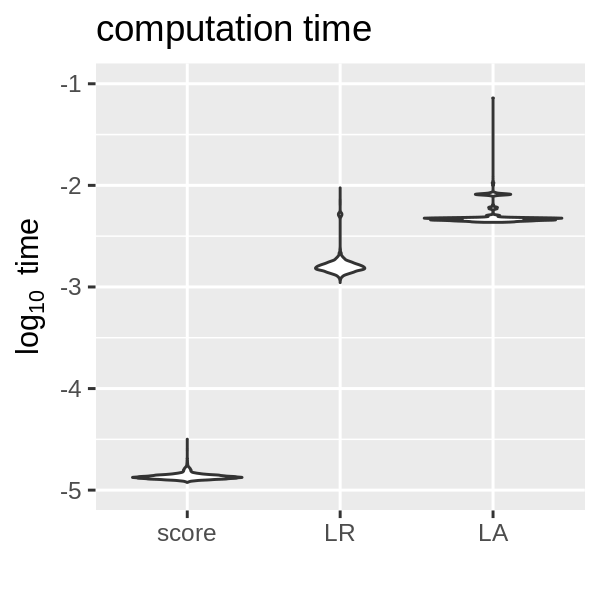
\includegraphics[width=0.32\textwidth]{figures/comptime.png}
        \includegraphics[width=0.32\textwidth]{figures/comptime_2020_01_12.png}
        \caption{The first and second plots show the two example functions $\rho$ used to generate data. The third plot shows for each method the distribution of the 1000 separate run-times for computing a single score test. The proposed method performs better than likelihood ratio test in the scale of $10^2$.}
        \label{fig:sim}
\end{figure}

Table \ref{tab:pairwise_simulation} summarizes the result. It counts the proportion of simulations which showed $p$-values less than 0.05 out of 1,000 total simulations. When $\rho$ is generated from hyperbolic tangent function, likelihood ratio test generally outperforms the other two methods, as expected, since the model is correctly specified in LR test. Score test, although it does not assume any model on $\rho$, does not lose as much power as liquid association does. Meanwhile, when $\rho$ is generated from quadratic function, score function clearly outperforms the other two methods. Hence, the simulations show that the proposed score test is robust to the shape of heteroskedasticity. Figure \ref{fig:sim} (c) shows the distribution of computation times of each method to compute the test statistic once in the scale of $log_{10}$ for 1000 simulations under quadratic model with $\alpha = 0.5$. The score test is the most efficient, because the likelihood ratio test requires numerical estimation of MLEs both under the null and under the alternative hypothesis while liquid association requires permutation test for inference. The simulations were done sequentially (non-parallel) with LAMBDA QUAD workstation with Intel Xeon W-2175 processor.

\begin{table}
\centering 
 \caption{Proportion of simulations for each method that showed $p$-value $<0.05$ at given data generating model and $\alpha$ level. We use two functions for $\rho$, hyperbolic tangent and quadratic function. The likelihood ratio test was conducted under the assumption that $\rho$ is hyperbolic tangent function.}
 \label{tab:pairwise_simulation}
\begin{tabular}{@{\extracolsep{5pt}} cc||cccc||cccc} 
\multicolumn{1}{c}{$\rho$} &\multicolumn{1}{c}{}& \multicolumn{4}{c}{tanh} & \multicolumn{4}{c}{quadratic}\\
\\[-1.8ex]\hline 
\hline \\[-1.8ex]
$\alpha$ & 0 & 0.25 & 0.5 & 0.75 & 1 & 0.2 & 0.3 & 0.4 & 0.5\\ 
\hline \\[-1.8ex]
score & 0.052 & 0.181 & 0.467 & 0.806 & 0.928 & 0.764 & 0.660 & 0.604 & 0.553\\
LA    & 0.051 & 0.181 & 0.472 & 0.779 & 0.911 & 0.048 & 0.054 & 0.054 & 0.052\\
LR    & 0.056 & 0.199 & 0.544 & 0.885 & 0.979 & 0.643 & 0.472 & 0.398 & 0.344\\
\\[-1.8ex]\hline 
\hline \\[-1.8ex]
\end{tabular}
\end{table} 

\section{Applications to GTEx Data} \label{sec:applications}
We next apply this method to 71 African American samples from GTEx \cite{gtex2015genotype} whose expression level data for muscle skeletal tissue is available. We aim to find transcription factors that change their coexpression pattern with their target genes as the genome's proportion of African ancestry changes. We acquire a list of transcription factors from TF checkpoint database  in \cite{chawla2013tfcheckpoint}. We also acquire a list of target genes for each transcription factors from TF2DNA database in \cite{pujato2014prediction}. We only take into consideration target genes with the highest binding scores. We use the proportion of African ancestry for each individual as the covariate, and it is inferred from the genotype data using the software LAMP  by \cite{pacsaniuc2009imputation}. The proportion of African ancestry levels from the subjects range from 14\% to 96\%.\\ 

For each of the $k = 1, \cdots, K = 848$ transcription factor encoding gene, we compute the pair-wise statistic $q_{kj}$ for all its target genes $j = 1, \cdots, J_k$, where $J_k$ is the number of target genes for each transcription factor $k$. Then, we compute $d_k = \sum_{j=1}^{J_k} q_{kj}$ to test the hypothesis that the correlation between the transcription factor $k$ and its targets remain the same across different genetic industry. We first divide $d_k$ with the number of targets $J_k$ to compute the average score of all the target genes for the given TF $k$, and we make a heuristic comparison against $\chi_1^2$ distribution. Under the null hypothesis, the expectation of $d_k/J_k$ is 1, although the variance is not trivial due to high dependence. Then, we choose 10 genes with the top $d_{k}/J_k$ values to perform the permutation test. \\

Table \ref{tab:results} summarizes the top 5 transcription factors with the highest average $d_k$ values and their $p$-values computed from sequential permutation tests. The adjusted $p$-values were computed by
$$\text{adjusted } p = p \times (\text{number of transcription factors}) / (\text{rank of $p$}).$$

\begin{table}[!htbp] \centering 
\begin{tabular}{@{\extracolsep{5pt}} ccc} 
\\[-1.8ex]\hline 
\hline \\[-1.8ex] 
Gene Name & $p$-value & Adjusted $p$-value \\ 
\hline \\[-1.8ex] 
MECOM & $< 10^{-5}$ & $< 0.01$ \\ 
ZNF423 & $< 10^{-5}$ & $< 0.01$ \\ 
SPIB & 0.001 & 0.326 \\ 
ZNF618 & 0.002 & 0.339 \\ 
ZSCAN & 0.002 & 0.415 \\ 
% ZNF136 & 0.003 & 0.424 \\ 
\hline \\[-1.8ex] 
\end{tabular} 
\caption{ Top 5 transcription factors with the lowest $p$-value  \label{tab:results} } 
\end{table} 
\noindent Two genes, MECOM and ZNF423, maintain their significance level of 0.01 under the Bonferroni criterion for 912 transcription factors. For the top gene MECOM, the two highest contributing target genes were C3orf70 and P2RY1, each having scores of 26.74 and 25.69 (should follow $\chi_1^2$ under the null hypothesis). Although these values look very high, they do not pass the Bonferroni test after taking into account the number of tests. The significance of MECOM (and ZNF423) is achieved through combining the scores across all the target genes. 

\section{Discussion}
We proposed a method to test whether the covariance between bivariate normal variables changes with continuous covariates. We further expanded our scope of analysis by looking at local connectivity --- how one variable's connectivity with multiple other variables change with continuous covariates. We provided a real data example by identifying major transcription factor genes that are differentially connected with its targets by African Americans' genetic ancestry. \\

Our method is more flexible than other alternatives for covariance testing, but it still has some limitations. First, when there are more variables than the available sample size, as often is the case for many modern data sets, we ultimately turn to a permutation test, not being able to take the computational advantage of the theoretical results. There could be other ways, depending on contexts, to estimate $\Sigma$ to avoid the permutation test. For example, one could impose the sparsity assumption on the covariance matrix, and that can lead to a reliable estimate of $\Sigma$ and subsequently $H$ in (\ref{eq:H}). Such assumption is too restrictive in our context, but in other applications, one can take the liberty to make structural assumptions on the covariance matrix. Nonetheless, it is challenging, to say the least, to find consistent estimators for the eigenvalues of $\Sigma$ in high-dimensional data. Second, the score statistic $q$ was derived under the normality assumption of the data set, although simulations show that the result is quite robust to distribution mis-specification. These limitations of the methods propose possible future research topics: (1) better way to estimate $H$ in (\ref{eq:H}) when $K > N$ to preserve asymptotic results, and (2) a non-parametric version of correlation analysis that can generalize to any underlying distributions. \\

In practice, users of this method should note the method's sensitivity to correct mean modeling. For example, if correct data generating procedure is $\bm{z}_i = \bm{x}_i$ + $\bm{x}_i^2$, missing the quadratic term (mis-specifying $\bm{z}_i$ as $\bm{x}_i$) would incorrectly assign the effects of $\bm{x}_i^2$ to the residuals. Then, the score statistic computed from the residuals will have some remaining effects from the mean term, and hence the type I error will be inflated. Therefore, the users are expected to be careful in regressing out all the relevant terms so that the mean term effects do not spill over to the variance term.\\ 

We believe the proposed method can be applied to data problems in diverse domains, especially where certain hub variables are connected to many other variables as in the transcriptional regulatory network. Many network problems, such as protein interactions, metabolic networks, co-authorship network, and semantic network, are known to have, or have something close to, scale-free topology, indicating that the important variables in those networks can be tested against other variables. The proposed correlation analysis will provide insights into the building blocks of diverse network problems by looking at the pairwise and more than pairwise relationships among the variables.

\bibliographystyle{imsart-nameyear}
\bibliography{ref}
 
\pagebreak
 
\section*{Appendix A. Derivation of test statistic}
% We start from the model in (\ref{eq:framework_2genes}). 
Consider the likelihood in (\ref{eq:likelihood_2genes}).
\begin{equation}
\begin{multlined}
\ell(\bm{\alpha}, \alpha_0, \bm{b}, \bm{\beta}, \rho_{11}, \rho_{22}) 
% = -\frac{N}{2} log(2\pi) - \frac{1}{2} \sum_{i=1}^{N} log (\sigma_{wi}^2) - \sum_{i=1}^{N} \frac{(w_i - \mu_{wi})^2}{\sigma_{wi}^2}\\
% \hspace{7mm} -\frac{N}{2} log(2\pi) - \frac{1}{2} \sum_{i=1}^{N} log (\sigma_{vi}^2) - \sum_{i=1}^{N} \frac{(v_i - \mu_{vi})^2}{\sigma_{vi}^2}\\
= -N log(2\pi) \\ - \frac{1}{2} \sum_{i=1}^{N} log(\sigma_{wi}^2) - \frac{1}{2} \sum_{i=1}^{N} log(\sigma_{vi}^2) - \sum_{i=1}^{N} \frac{u_{wi}^2}{2\sigma_{wi}^2} - \sum_{i=1}^{N} \frac{u_{vi}^2}{2\sigma_{vi}^2}
\end{multlined}
    \label{eq:likelihood_2genes_appendix}
\end{equation}
% $$\mu_{wi} = \frac{{b}_1}{\sqrt{\rho_{11}}} + \frac{{b}_2}{\sqrt{\rho_{22}}} + \bm{x}_i^T \left(\frac{\bm{\beta}_1}{\sqrt{\rho_{11}}} + \frac{\bm{\beta}_2}{\sqrt{\rho_{22}}}\right), \hspace{6mm} 
% \mu_{vi} = \frac{{b}_1}{\sqrt{\rho_{11}}} - \frac{{b}_2}{\sqrt{\rho_{22}}} + \bm{x}_i^T \left(\frac{\bm{\beta}_1}{\sqrt{\rho_{11}}} - \frac{\bm{\beta}_2}{\sqrt{\rho_{22}}}\right)$$
% $$\sigma_{wi}^2 = 2 + \frac{2\rho_{12}(\bm{x}_i^T\bm{\alpha} + \alpha_0)}{\sqrt{\rho_{11}\rho_{22}}}, \hspace{6mm} \sigma_{vi}^2 = 2 - \frac{2\rho_{12}(\bm{x}_i^T\bm{\alpha} + \alpha_0)}{\sqrt{\rho_{11}\rho_{22}}}$$

We compute the first and second derivative of the log likelihood with respect to $\bm{\alpha}$ when all other nuisance parameters are replaced with their respective maximum likelihood estimates. The following results help the computation of the derivative.
$$
\frac{\partial \sigma_{wi}^2}{\partial \bm{\alpha}} = \frac{2\bm{x}_i \rho_{12}'(\bm{x}_i^T \bm{\alpha} + \alpha_0)}{\sqrt{\rho_{11}\rho_{22}}}, \hspace{5mm}
\frac{\partial \sigma_{vi}^2}{\partial \bm{\alpha}} = -\frac{2\bm{x}_i \rho_{12}'(\bm{x}_i^T \bm{\alpha} + \alpha_0)}{\sqrt{\rho_{11}\rho_{22}}}
$$
$$\frac{\partial \sigma_{wi}^2}{\partial \rho_{11}} = -\frac{\rho_{12}(\bm{x}_i^T\bm{\alpha} + \alpha_0)}{\sqrt{\rho_{11}^3\rho_{22}}} = \frac{1}{\rho_{11}}\left(-\frac{\sigma_{wi}^2}{2} + 1\right)$$
$$\frac{\partial \sigma_{vi}^2}{\partial \rho_{11}} = \frac{\rho_{12}(\bm{x}_i^T\bm{\alpha} + \alpha_0)}{\sqrt{\rho_{11}^3\rho_{22}}} = \frac{1}{\rho_{11}}\left(\frac{\sigma_{vi}^2}{2} - 1\right)$$

% \noindent We additionally define $\hat{u}_{wi}^2$ and $\hat{v}_{wi}^2$ as $(w_i - \hat{\mu}_{wi})^2$ and $(v_i-\hat{\mu}_{vi})^2$ respectively, where $\hat{\mu}_{wi}$ and $\hat{\mu}_{vi}$ are $\mu_{wi}$ and $\mu_{vi}$ with $\bm{b}$ and $\bm{\beta}$ replaced with $\hat{\bm{b}}$ and $\hat{\bm{\beta}}$.\\

\noindent The maximum likelihood estimates for $\sigma_{wi}^2$ and $\sigma_{vi}^2$ are as follows.
$$\hat{\sigma}_{wi}^2 = \frac{1}{N} \sum_{i=1}^{N} \hat{u}_{wi}^2, \hspace{5mm} 
\hat{\sigma}_{wi}^2 = \frac{1}{N} \sum_{i=1}^{N} \hat{u}_{vi}^2$$
Then, the first derivative of the likelihood (\ref{eq:likelihood_2genes_appendix}) with respect to the parameter of interest $\bm{\alpha}$ is
\begin{equation}
    \begin{multlined}
    \bm{d}_{\bm{\alpha}} = \frac{\partial \ell}{\partial \bm{\alpha}} = - \sum_{i=1}^{N} \frac{1}{2\sigma_{wi}^2} \cdot \frac{\partial \sigma_{wi}^2}{\partial \bm{\alpha}} - \sum_{i=1}^{N} \frac{-(w_i - \mu_{wi})^2}{2\sigma_{wi}^4} \frac{\partial \sigma_{wi}^2}{\partial \bm{\alpha}}\\
    - \sum_{i=1}^{N} \frac{1}{2\sigma_{vi}^2} \cdot \frac{\partial \sigma_{vi}^2}{\partial \bm{\alpha}} - \sum_{i=1}^{N} \frac{-(v_i - \mu_{vi})^2}{2\sigma_{vi}^4} \frac{\partial \sigma_{vi}^2}{\partial \bm{\alpha}}\\
    =-\frac{1}{\sqrt{\rho_{11}\rho_{22}}} \sum_{i=1}^{N} \bm{x}_i \rho_{12}'(\bm{x}_i^T\bm{\alpha} + \alpha_0) \cdot \left(
    \frac{1}{\sigma_{wi}^2} - \frac{u_{wi}^2}{\sigma_{wi}^4} 
    - \frac{1}{\sigma_{vi}^2} + \frac{u_{vi}^2}{\sigma_{vi}^4}
    \right)\\
    = -\frac{1}{\sqrt{\rho_{11}\rho_{22}}} \sum_{i=1}^{N} \bm{x}_i\rho_{12}'(\bm{x}_i^T \bm{\alpha}+\alpha_0) \cdot 
    \left(
    \frac{1}{\sigma_{wi}^2} \left( 1 - \frac{u_{wi}^2}{\sigma_{wi}^2}\right) - 
    \frac{1}{\sigma_{vi}^2} \left( 1 - \frac{u_{vi}^2}{\sigma_{vi}^2} \right)
    \right).
    \end{multlined}
\end{equation}
\noindent Plugging in $\bm{0}$ for $\bm{\alpha}$ and maximum likelihood estimators for all nuisance parameters, we get the score function as below. 
\begin{equation}
    \begin{multlined}
    \bm{\tilde{d}}_{\bm{\alpha}} = \bm{d}_{\bm{\alpha}}\mid_{\bm{\alpha}=\bm{0}, \alpha_0 = \hat{\alpha}_0, \bm{b} = \bm{\hat{b}},\bm{\beta} = \bm{\hat{\beta}}, {\rho}_{11} = {\bm{\hat{\rho}}_{11}},
    {\rho}_{22} = {\bm{\hat{\rho}}_{22}}}\\
    = -\frac{\rho_{12}'(\hat{\alpha}_0)}{\sqrt{\rho_{11}\rho_{22}}} \sum_{i=1}^{N} \frac{\bm{x}_i}{\hat{\sigma}_{w}^2} - \frac{\bm{x}_i}{\hat{\sigma}_{v}^2} - \frac{\bm{x}_i \hat{u}_{wi}^2}{\hat{\sigma}_{wi}^4} + \frac{\bm{x}_i \hat{u}_{v}^2}{\hat{\sigma}_{v}^4}\\
    = -\frac{\rho_{12}'(\hat{\alpha}_0)}{\sqrt{\rho_{11}\rho_{22}}} \sum_{i=1}^{N} \left(
    \frac{\bm{x}_i}{\hat{\sigma}_{w}^2}
    \left( 1-\frac{\hat{u}_{wi}^2}{\hat{\sigma}_{w}^2}\right) - 
    \frac{\bm{x}_i}{\hat{\sigma}_{v}^2}
    \left( 1-\frac{\hat{u}_{vi}^2}{\hat{\sigma}_{v}^2}\right) 
    \right)
    \end{multlined}
\end{equation}

% \begin{align*}
% \bm{d}_{\bm{\alpha}} &= \frac{\partial \ell}{\partial \bm{\alpha}}\\
% &= -\frac{1}{2} \sum_{i=1}^{N}  \frac{2\rho'(\bm{x}_i^T \bm{\alpha})\bm{x}_i}{\sigma_{wi}^2} \left(
% 1 - \frac{u_{wi}^2}{\sigma_{wi}^2} 
% \right) + \frac{1}{2} \sum_{i=1}^{N}\frac{2\rho'(\bm{x}_i^T \bm{\alpha})\bm{x}_i}{\sigma_{vi}^2} \left(
% 1 - \frac{u_{vi}^2}{\sigma_{vi}^2}\right).
% \end{align*}

%  Now, we replace $\bm{\beta}$ and $\bm{\alpha}$ with the maximum likelihood estimators under the null hypothesis. $\bm{\beta}$ is therefore replaced by the OLS estimators, and $\bm{\alpha}$ is 0. Moreover, the MLE for
% $2 + 2\rho(\bm{0}) = \hat{\sigma}_w^2$ and MLE for $2-2\rho(\bm{0}) = \hat{\sigma}_v^2$. 
% \begin{equation}
%     \begin{multlined}
% \bm{\tilde{d}_{\alpha}} = \bm{d}_{\bm{\alpha}}\mid_{\bm{\alpha}=\bm{0}, \bm{\beta} = \bm{\hat{\beta}}_{\text{MLE}}} \\
% = -\frac{1}{2} \sum_i \left(
% \frac{2\rho'(0)\bm{x}_i}{\hat{\sigma}_{w}^2} \left(
% 1-\frac{\hat{u}_{wi}^2}{\hat{\sigma}_{w}^2}
% \right)
% -
% \frac{2\rho'(0)\bm{x}_i}{\hat{\sigma}_{v}^2} \left(
% 1-\frac{\hat{u}_{vi}^2}{\hat{\sigma}_{v}^2}
% \right)
% \right)\\
% = -\rho'(0) \sum_i  \left(
% \frac{\bm{x}_i}{\hat{\sigma}_{w}^2} \left(
% 1-\frac{\hat{u}_{wi}^2}{\hat{\sigma}_{w}^2}
% \right)
% -
% \frac{\bm{x}_i}{\hat{\sigma}_{v}^2} \left(
% 1-\frac{\hat{u}_{vi}^2 }{\hat{\sigma}_{v}^2}
% \right)
% \right)
% \label{first_derivative}
% \end{multlined}
% \end{equation}
\noindent The second derivative is
\begin{equation}
    \begin{multlined}
    \frac{\partial^2 \ell}{\partial \bm{\alpha} \partial \bm{\alpha}^T}\\
    = \sum_{i=1}^{N} \frac{\bm{x}_i \bm{x}_i^T \rho_{12}''(\bm{x}_i^T\bm{\alpha}+\alpha_0)}{\sqrt{\rho_{11}\rho_{22}}} \cdot
    \left(
    \frac{1}{\sigma_{wi}^2} \left( 1 - \frac{u_{wi}^2}{\sigma_{wi}^2}\right) - 
    \frac{1}{\sigma_{vi}^2} \left( 1 - \frac{u_{vi}^2}{\sigma_{vi}^2} \right)
    \right)\\
    + \frac{2\bm{x}_i \bm{x}_i^T {\rho_{12}'}^2(\bm{x}_i^T\bm{\alpha} + \alpha_0)}{\rho_{11}\rho_{22}}
    \left(
    -\frac{1}{\sigma_{wi}^4} + \frac{2u_{wi}^2}{\sigma_{wi}^6} +
    -\frac{1}{\sigma_{vi}^4} + \frac{2u_{vi}^2}{\sigma_{vi}^6}
    \right)\\
    = \sum_{i=1}^{N} \frac{\bm{x}_i \bm{x}_i^T \rho_{12}''(\bm{x}_i^T\bm{\alpha}+\alpha_0)}{\sqrt{\rho_{11}\rho_{22}}} \cdot
    \left(
    \frac{1}{\sigma_{wi}^2} \left( 1 - \frac{u_{wi}^2}{\sigma_{wi}^2}\right) - 
    \frac{1}{\sigma_{vi}^2} \left( 1 - \frac{u_{vi}^2}{\sigma_{vi}^2} \right)
    \right)\\
    - \frac{2\bm{x}_i \bm{x}_i^T {\rho_{12}'}^2(\bm{x}_i^T\bm{\alpha}+\alpha_0)}{\rho_{11}\rho_{22}}
    \left(
    \frac{1}{\sigma_{wi}^4} \left(1-\frac{2u_{wi}^2}{\sigma_{wi}^2}\right)+
    \frac{1}{\sigma_{vi}^4} \left(1-\frac{2u_{vi}^2}{\sigma_{vi}^2}\right)
    \right).
    \end{multlined}
\end{equation}
We acquire the Fisher Information matrix by taking an expectation:
\begin{equation}
    \mathcal{I}_{\bm{\alpha}\bm{\alpha}^T} = E\left(\frac{\partial^2 \ell}{\partial \bm{\alpha} \partial \bm{\alpha}^T}\right)\\
    = \sum_{i=1}^{N} \frac{2\bm{x}_i \bm{x}_i^T {\rho '}^2_{12}(\bm{x}_i^T\bm{\alpha}+\alpha_0)}{\rho_{11}\rho_{22}} \left(
    \frac{1}{\sigma_{wi}^4} + \frac{1}{\sigma_{vi}^4}
    \right).
\end{equation}

\noindent Then we plug in the maximum likelihood estimates as follows.
\begin{equation}
\begin{multlined}
        \tilde{\mathcal{I}}_{\bm{\alpha}\bm{\alpha}^T} = \mathcal{I}_{\bm{\alpha}\bm{\alpha}^T}\mid_{
        \bm{\alpha}=\bm{0}, 
        \alpha_0 = \hat{\alpha}_0,
        \bm{b} = \bm{\hat{b}},
        \bm{\beta} = \bm{\hat{\beta}},
        {\rho}_{11} = \bm{\hat{\rho}}_{11},
        {\rho}_{22} = \bm{\hat{\rho}}_{22}}\\
        = \frac{{\rho '}^2_{12}({\hat{\alpha}_0})}{2\hat{\rho}_{11}\hat{\rho}_{22}} \left(\frac{1}{\hat{\sigma}_{w}^4} + \frac{1}{\hat{\sigma}_{v}^4} \right) \sum_{i=1}^{N} \bm{x}_i \bm{x}_i^T
    \end{multlined}
\end{equation}

\noindent Additionally, we can see that $\tilde{\mathcal{I}}_{\bm{\alpha}{\bm{\beta}_1^T}} =  \tilde{\mathcal{I}}_{\bm{\alpha}{\bm{\beta}_2^T}} = \bm{0}$
\begin{equation}
\frac{\partial \ell}{\partial \bm{\alpha} \partial\bm{\beta}_1}= 
    % {\mathcal{I}}_{\bm{\alpha}{\bm{\beta}_1^T}} =
    \frac{1}{\sqrt{\rho_{11}\rho_{22}}} \sum_i \bm{x}_i \bm{x}_i^T \rho_{12}(\bm{x}_i^T\bm{\alpha} + \alpha_0) \left( 
    \frac{u_{wi}}{\sqrt{\rho_{11}}\sigma_{wi}^4} + \frac{u_{vi}}{\sqrt{\rho_{11}}\sigma_{vi}^4}
    \right)
\end{equation}
$$
\tilde{\mathcal{I}}_{\bm{\alpha}{\bm{\beta}_1^T}} = 
\frac{\rho_{12}(\hat{\alpha}_0)}{\sqrt{\hat{\rho}_{11}^3\hat{\rho}_{22}}} \left(
\frac{1}{\hat{\sigma}_{wi}^4}
E\left( \sum_{i=1}^{n} \bm{x}_i \bm{x}_i^T \hat{u}_{wi}\right)
+\frac{1}{\hat{\sigma}_{vi}^4}
E\left( \sum_{i=1}^{n} \bm{x}_i \bm{x}_i^T \hat{u}_{vi} \right)
\right) = \bm{0}$$

% \noindent $\tilde{\mathcal{I}}_{\bm{\alpha}\bm{\rho}_{11}}$ is
% \begin{equation}
%     \begin{multlined}
%     \frac{\partial \ell}{\partial \bm{\alpha}\partial\rho_{11}} = \\
%      \sum_{i=1}^{N} -\frac{\bm{x}_i \rho'_{12}(\bm{x}_i^T \bm{\alpha}+\alpha_0)}{2\sqrt{\rho_{11}^3\rho_{22}}} \left( \frac{1}{\sigma_{wi}^2}\left( 1-\frac{u_{wi}^2}{\sigma_{wi}^2} \right) - 
%      \frac{1}{\sigma_{vi}^2} \left( 1-\frac{u_{vi}^2}{\sigma_{vi}^2}\right) \right)\\
%      + \frac{\bm{x}_i \rho_{12}(\bm{x}_i^T\bm{\alpha} + \alpha_0) \rho_{12}'(\bm{x}_i^T \bm{\alpha} + \alpha_0)}{2\rho_{11}^2 \rho_{22}}\left( \frac{1}{\sigma_{wi}^4}\left( 1-\frac{u_{wi}^2}{2\sigma_{wi}^2} \right) - 
%      \frac{1}{\sigma_{vi}^4} \left( 1-\frac{u_{vi}^2}{2\sigma_{vi}^2}\right) \right).
%     \end{multlined}
% \end{equation}

\noindent Next, we compute $\tilde{\mathcal{I}}_{\bm{\alpha}\bm{\rho}_{11}}$.
\begin{equation}
    \begin{multlined}
    \frac{\partial \ell}{\partial \bm{\alpha}\partial\rho_{11}} = \\
    \frac{1}{2\sqrt{\rho_{11}^3\rho_{22}}} \sum_{i=1}^{N} \bm{x}_i \rho_{12}'(\bm{x}_i^T\bm{\alpha}+\alpha_0) (A-B)\\
    - \frac{1}{\sqrt{\rho_{11}\rho_{22}}} \sum_{i=1}^{N} \bm{x}_i \rho_{12}'(\bm{x}_i^T\bm{\alpha} + \alpha_0) \left( \frac{\partial A}{\partial \rho_{11}} - \frac{\partial B}{\partial \rho_{11}}\right)
    \end{multlined}
    \end{equation}
where $A = \frac{1}{\sigma_{wi}^2} \left( 1 - \frac{u_{wi}^2}{\sigma_{wi}^2}\right)$ and $B = \frac{1}{\sigma_{vi}^2} \left( 1-\frac{u_{vi}^2}{\sigma_{vi}^2}\right)$. The first term is zero under the null with nuisance parameters replaced with MLEs. After some computation,
$$\frac{\partial A}{\partial \rho_{11}} =  \frac{1}{(\sigma_{wi}^2)^2\rho_{11}},\hspace{6mm}
\frac{\partial B}{\partial \rho_{11}} =  \frac{1}{(\sigma_{vi}^2)^2\rho_{11}}$$
Under the null with nuisance parameters replaced with MLEs,
$$\tilde{\mathcal{I}}_{\bm{\alpha}\rho_{11}} = 
-\frac{\rho_{12}'(\hat{\alpha}_0)}{\sqrt{\hat{\rho}_{11}^3\hat{\rho}_{22}}} \left(\frac{1}{\hat{\sigma}_w^4} - \frac{1}{\hat{\sigma}_v^4} \right)\sum_{i=1}^{N} \bm{x}_i 
,
$$
which is $\bm{0}$ under the small condition that the covariates are centered so that $\sum_{i=1}^{N}\bm{x}_i = \bm{0}$. $\tilde{\mathcal{I}}_{\bm{\alpha}\rho_{22}}$ is similar due to symmetry.\\




%%%%%%% DETAILED DERIVATION OF $\frac{\partial A}{\partial \rho_{11}}$ %%%%%
%%%%%%% DO NOT DELETE %%%%%%
% The first term above is zero under the null with nuisance parameters replaced with MLEs. For the second term, we first compute $\frac{\partial A}{\partial \rho_{11}}:$
% $$\frac{\frac{\partial \sigma_{wi}^2}{\partial \rho_{11}}}{(\sigma_{wi}^2)^2} \left( 1 - \frac{u_{wi}^2}{\sigma_{wi}^2} \right) + \frac{1}{\sigma_{wi}^2} \left(
% -\frac{2u_{wi} \frac{\partial u_{wi}}{\partial \rho_{11}} \sigma_{wi}^2 - u_{wi}^2 \frac{\partial \sigma_{wi}^2}{\partial \rho_{11}}}{(\sigma_{wi}^2)^2}
% \right)$$
% The first term becomes zero under the null with MLEs of nuisance parameters. The second term can be re-written as
% $$
% -\frac{-\frac{u_{1i}^2}{\rho_{11}} - \frac{u_{1i}u_{2i}}{\sqrt{\rho_{11}\rho_{22}}}}{(\sigma_{wi}^2)^2\rho_{11}}
% - \frac{\frac{\rho_{12}(\bm{x}_i^T\bm{\alpha} + \alpha_0)}{\sqrt{\rho_{11}\rho_{22}}} \cdot u_{wi}^2}{(\sigma_{wi}^2)^3\rho_{11}}
% $$

% \noindent Taking expectation,
% $$\frac{1}{(\sigma_{wi}^2)^2\rho_{11}} + \frac{\frac{\rho_{12}(\bm{x}_i^T\bm{\alpha} + \alpha_0)}{\sqrt{\rho_{11}\rho_{22}}}}{(\sigma_{wi}^2)^2\rho_{11}}  - \frac{\frac{\rho_{12}(\bm{x}_i^T\bm{\alpha} + \alpha_0)}{\sqrt{\rho_{11}\rho_{22}}}}{(\sigma_{wi}^2)^2\rho_{11}}$$
% $$= \frac{1}{(\sigma_{wi}^2)^2\rho_{11}} $$

% \noindent Plugging in the MLEs of the nuisance parameters,
% $$\frac{1}{\hat{\sigma}_w^4\hat{\rho}_{11}}$$

% Going back to the original expression,
% $$E\left(\frac{\partial \ell}{\partial \bm{\alpha} \partial \rho_{11}}\right)\mid_{
%         \bm{\alpha}=\bm{0}, 
%         \alpha_0 = \hat{\alpha}_0,
%         \bm{b} = \bm{\hat{b}},
%         \bm{\beta} = \bm{\hat{\beta}},
%         {\rho}_{11} = \bm{\hat{\rho}}_{11},
%         {\rho}_{22} = \bm{\hat{\rho}}_{22}} =\tilde{\mathcal{I}}_{\bm{\alpha}\bm{\rho}_{11}}$$
% $$= \frac{\rho_{12}'(\hat{\alpha}_0)}{2\sqrt{\hat{\rho}_{11}^3\hat{\rho}_{22}}} \sum_i \bm{x}_i \left( 1 - \frac{E(\hat{u}_{wi}^2)}{\hat{\sigma}_{w}^2} - 1 + \frac{E(\hat{u}_{vi}^2)}{\hat{\sigma}_{v}^2} \right)
% $$
% $$- \frac{\rho_{12}'(\hat{\alpha}_0)}{\sqrt{\hat{\rho}_{11}^3\hat{\rho}_{22}}}
% \sum_i \bm{x}_i \left( \frac{1}{\hat{\sigma}_w^4\hat{\rho}_{11}} + \frac{1}{\hat{\sigma}_v^4 \hat{\rho}_{22}} \right)
% $$
% $$=-\frac{\rho_{12}'(\hat{\alpha}_0)}{\sqrt{\rho_{11}^3 \rho_{22}}} \sum_{i=1}^{N} \bm{x}_i \left( \frac{1}{\hat{\sigma}_w^2}\left( \frac{3}{\hat{\sigma}_w^2} - \frac{1}{2} \right) - \frac{3}{\hat{\sigma}_v^2} \left( \frac{1}{\hat{\sigma}_v^2} - \frac{1}{2} \right) \right)$$
% and $\tilde{\mathcal{I}}_{\bm{\alpha}\bm{\rho}_{22}}$ is similar. We can see that above equals to zero under a small condition that the covariates are centered. The centering of covariates plays no role in inference. \\

\noindent Finally, we get our score statistic
\begin{equation}
    \begin{multlined}
    q = \tilde{d}_{\bm{\alpha}}^T \tilde{I}_{\bm{\alpha}\bm{\alpha}^T}^{-1}
    \tilde{d}_{\bm{\alpha}}
    =\frac{1}{2}\left( \frac{1}{\hat{\sigma}_w^4}+\frac{1}{\hat{\sigma}_v^4}\right)^{-1}
\left(\sum_{i=1}^{N} \bm{x}_{i} 
\left(
\frac{\hat{\sigma}_w^2-\hat{u}_{wi}^2}{\hat{\sigma}_w^4}- \frac{\hat{\sigma}_v^2-\hat{u}_{vi}^2}{\hat{\sigma}_v^4}
\right)
\right)^T \\
\left( \sum_{i=1}^{N} \bm{x}_i^T \bm{x}_i \right)^{-1}
\left(
\sum_{i=1}^{N} \bm{x}_{i} 
\left(
\frac{\hat{\sigma}_w^2-\hat{u}_{wi}^2}{\hat{\sigma}_w^4}- \frac{\hat{\sigma}_v^2-\hat{u}_{vi}^2}{\hat{\sigma}_v^4}
\right)
\right)
    \end{multlined}
\end{equation}


\section*{Appendix B. Derivation of $\eta_{12,13}$}
We start from the test statistic $q$ computed when the covariates have been orthogonalized.
$$q = \sum_{p=1}^{P}
 \left(\frac{1}{\sqrt{N}}
 \sqrt{\frac{\hat{\sigma}_w^4 \hat{\sigma}_v^4}{\hat{\sigma}_w^4 + \hat{\sigma}_v^4}}
 \sum_{i=1}^{N} x_{ip} \left( \frac{\hat{\sigma}_w^2 - \hat{u}_{wi}^2}{\hat{\sigma}_w^4}
 - \frac{\hat{\sigma}_v^2 - \hat{u}_{vi}^2}{\hat{\sigma}_v^4}
 \right)
\right)^2 = \sum_{p=1}^{P}r_p^2$$
$r_p$ for each $p$ follows standard normal distribution by the central limit theorem. 
$$E\left(x_{ip}\left( \frac{\hat{\sigma}_w^2 - \hat{u}_{wi}^2}{\hat{\sigma}_w^4}
 - \frac{\hat{\sigma}_v^2 - \hat{u}_{vi}^2}{\hat{\sigma}_v^4}
 \right)\right) = x_{ip} E\left( \frac{\hat{\sigma}_w^2 - \hat{u}_{wi}^2}{\hat{\sigma}_w^4} \right) E\left( \frac{\hat{\sigma}_v^2 - \hat{u}_{vi}^2}{\hat{\sigma}_v^4}
 \right) = 0$$
$$Var\left(x_{ip}\left( \frac{\hat{\sigma}_w^2 - \hat{u}_{wi}^2}{\hat{\sigma}_w^4}
- \frac{\hat{\sigma}_v^2 - \hat{u}_{vi}^2}{\hat{\sigma}_v^4}
\right)\right) = 
x_{ip}^2 \left( Var\left( \frac{\hat{\sigma}_w^2 - \hat{u}_{wi}^2}{\hat{\sigma}_w^4} \right)  + Var\left( \frac{\hat{\sigma}_v^2 - \hat{u}_{vi}^2}{\hat{\sigma}_v^4}\right)\right)$$
 $$ = \frac{\hat{\sigma}_w^4 + \hat{\sigma}_v^4}{\hat{\sigma}_w^4 \hat{\sigma}_v^4}$$

\noindent We can re-write $r_{12,p}$ as following as a pre-processing to compute $cov(r_{12,p}, r_{12,p})$,
$$\hat{\sigma}_w^2 = 2 + \frac{2\hat{\rho}_{12}}{\sqrt{\hat{\rho}_{11}\hat{\rho}_{22}}} = 2+2\hat{\tau}_{12}$$
$$\hat{\sigma}_v^2 = 2 - \frac{2\hat{\rho}_{12}}{\sqrt{\hat{\rho}_{11}\hat{\rho}_{22}}} = 2-2\hat{\tau}_{12}$$
where $\rho_{12}$ is the constant correlation between variables 1 and 2 under the null hypothesis. Note that $\hat{\sigma}_w^2$ converges to $\sigma_w^2$ in probability, and so does $\hat{\rho}_{12}$ to $\rho_{12}$. We also define
$\hat{\tau}_{13} = \frac{\hat{\rho}_{13}}{\sqrt{\hat{\rho}_{11}\hat{\rho}_{33}}}$
$\hat{\tau}_{23} = \frac{\hat{\rho}_{23}}{\sqrt{\hat{\rho}_{22}\hat{\rho}_{33}}}$
\begin{equation}
\begin{multlined}
    r_{p,12} = \frac{1}{\sqrt{2N}} \frac{1}{\sqrt{8(1 + \hat{\tau}_{12}^2)}}
    \sum_{i=1}^{N} x_{ip}\left( (2-2\hat{\tau}_{12})- \frac{2-2\hat{\tau}_{12}}{2+2\hat{\tau}_{12}}(\hat{u}_{1i}+\hat{u}_{2i})^2\right)\\  - \left( (2+2\hat{\tau}_{12}) - \frac{2+2\hat{\tau}_{12}}{2-2\hat{\tau}_{12}}(\hat{u}_{1i}-\hat{u}_{2i})^2\right)\\
    = \frac{1}{\sqrt{16N(1+\hat{\tau}_{12}^2)}} \sum_{i=1}^{N}x_{ip}
    \left( 
    \frac{4((\hat{\tau}_{12}^3 - \hat{\tau}_{12}) - \hat{u}_{1i}\hat{u}_{2i}(\hat{\tau}_{12}^2 + 1) + \hat{\tau}_{12}(\hat{u}_{1i}^2 + \hat{u}_{2i}^2))}{(1-\hat{\tau}_{12})(1+\hat{\tau}_{12})}
    \right)\\
    = \frac{1}{\sqrt{N(1+\hat{\tau}_{12}^2)}}\sum_{i=1}^{N}x_{ip} \left( 
    \frac{(\hat{\tau}_{12}^3 - \hat{\tau}_{12}) - \hat{u}_{1i}\hat{u}_{2i}(\hat{\tau}_{12}^2 + 1) + \hat{\tau}_{12}(\hat{u}_{1i}^2 + \hat{u}_{2i}^2)}{(1-\hat{\tau}_{12})(1+\hat{\tau}_{12})}
    \right)
\end{multlined}
\end{equation}

 Similarly,
\begin{align*}
    r_{p,13} = 
    \frac{1}{\sqrt{N(1+\hat{\tau}_{13}^2)}}\sum_{i=1}^{N}x_{ip} \left( 
    \frac{(\hat{\tau}_{13}^3 - \hat{\tau}_{13}) - \hat{u}_{1i}\hat{u}_{3i}(\hat{\tau}_{13}^2 + 1) + \hat{\tau}_{13}(\hat{u}_{1i}^2 + \hat{u}_{3i}^2))}{(1-\hat{\tau}_{13})(1+\hat{\tau}_{13})}
    \right)
\end{align*}

$$cov(r_{12,p}, r_{13,p}) = E(r_{12,p}r_{13,p}) - E(r_{12,p})E(r_{13,p}) = E(r_{12,p}r_{13,p})$$

 Then, after some algebra,

\begin{equation}
    \begin{multlined}
    \eta_{12,13} = E\sum_{i=1}^{N}x_{ip}^2  \frac{\hat{u}_{i1}^2 \hat{u}_{2i}\hat{u}_{3i}(\hat{\tau}_{12}^2+1)(\hat{\tau}_{13}^2+1)
    + \hat{\tau}_{12}\hat{\tau}_{13} (\hat{u}_{1i}^2 + \hat{u}_{2i}^2)(\hat{u}_{1i}^2 + \hat{u}_{3i}^2)}{N(1-\hat{\tau}_{12}^2)(1-\hat{\tau}_{13}^2)\sqrt{(1+\hat{\tau}_{12}^2)(1+\hat{\tau}_{13}^2)}} \\
    - \frac{\hat{\tau}_{12}(\hat{\tau}_{13}^2 + 1) (\hat{u}_{1i}\hat{u}_{3i})(\hat{u}_{1i}^2 + \hat{u}_{2i}^2) + \hat{\tau}_{13}(\hat{\tau}_{12}^2+1)(\hat{u}_{1i}\hat{u}_{2i})(\hat{u}_{1i}^2 + \hat{u}_{3i}^2)}{N(1-\hat{\tau}_{12}^2)(1-\hat{\tau}_{13}^2)\sqrt{(1+\hat{\tau}_{12}^2)(1+\hat{\tau}_{13}^2)}}
    \end{multlined} 
    \end{equation}
    
\begin{equation} \begin{multlined}
= \frac{(\tau_{23}+2\tau_{12}\tau_{13})(\tau_{12}^2+1)(\tau_{13}^2+1) + \tau_{12}\tau_{13}(6+2(\tau_{12}^2+\tau_{13}^2+\tau_{23}^2))}{(1-{\tau}_{12}^2)(1-{\tau}_{13}^2)\sqrt{(1+{\tau}_{12}^2)(1+{\tau}_{13}^2)}} \\
- \frac{\tau_{12}(\tau_{13}^2+1)(4\tau_{13}+2\tau_{12}\tau_{23}) + \tau_{13}(\tau_{12}^2+1)(4\tau_{12}+2\tau_{13}\tau_{23})}{(1-{\tau}_{12}^2)(1-{\tau}_{13}^2)\sqrt{(1+{\tau}_{12}^2)(1+{\tau}_{13}^2)}}
\end{multlined} \end{equation}
from
$$E(\hat{u}_{i1}^4) = 3, \hspace{5mm} E(\hat{u}_{i1}^3 \hat{u}_{i2}) = 3\tau_{12}, \hspace{5mm} E(\hat{u}_{i1}^2\hat{u}_{i2}^2) = 1 + 2\tau_{12}^2,$$
$$E(\hat{u}_{i1}^2 \hat{u}_{i2} \hat{u}_{i3}) = \tau_{23} + 2\tau_{12}\tau_{13}.$$

\section*{Appendix C. Details of Small Sample Correction}
Although the introduced test statistic $q$ asymptotically follows $\chi_1^2$, the statistic has its error in the order of $N^{-1}$ (\cite{harris1985asymptotic}) with finite sample size $N$, and many Monte Carlo experiments show that the test rejects the null hypothesis less frequently than indicated by its nominal size (\cite{godfrey1978testing, griffiths1986monte, honda1988size}). In response, Harris (1985) used Edgeworth expansion to obtain the distribution and moment generating function to order $N^{-1}$ of the test statistic (\cite{harris1985asymptotic}). Building on this expansion, Honda (1986) and Cribari-Neto and Ferrari (2001) proposed corrections to the critical value or to the test statistic that allows better inference even when the sample size is small while preserving the asymptotic properties.\\

Honda (1988) provided a closed-form formula to adjust the critical value in the order of $O(N^{-1})$ to correct the type I error of the test. This adjustment, only depending on the covariate, sample size, and the degrees of freedom, but not on the data, is a cubic function with respect to $C_{\gamma}$, the critical value at the level of type I error $\gamma$, i.e. $P(\chi_{P}^2 \geq C_{\gamma}) = \gamma$, and we refer to this cubic function as $g$ defined as follows.

\begin{equation}
    \begin{multlined}
g(C_{\gamma}) = C_{\gamma} + C_{\gamma}\bigg(\frac{A_3 - A_2 + A_1}{12NP}\bigg) + C_{\gamma}^2\bigg(\frac{A_2 - 2A_3}{(12NP(P+2)}\bigg) +\\
C_{\gamma}^3 \bigg(\frac{A_3}{12NP(P+2)(P+4)}\bigg) = C_{\gamma} + \tilde{g}(C_{\gamma})
\end{multlined}
\label{eq:hondacorrection}
\end{equation}

where the scalars $A_1$, $A_2$, and $A_3$ follow the notation of Honda (1988) directly. 

\vspace{5mm}  
One of the desirable properties of $g$ would be monotonicity, because regardless of sample size, we would like to maintain the same ordering of the strength of evidence against the null. This turns out to be almost always true in practice. The derivative of $g(C)$ is 
$$g'(C_{\gamma}) = \frac{A_3}{12NP}\left( \frac{A_3-A_2+A_1+12NP}{A_3} + 
 \frac{2(A_2-2A_3)}{(P+2)A_3}C_{\gamma} + \frac{3}{(P+2)(P+4)}C_{\gamma}^2 \right)$$
$A_3$ is strictly positive by definition, and we can solve the above quadratic equation to see in which case the derivative is positive (\cite{cribari1995improved}). In other words, we can study when the following discriminant is complex.
$$\sqrt{\left(\frac{2(A_2-2A_3)^2}{(P+2)A_3}\right)^2 - 4\cdot\frac{3A_3(A_3-A_2+A_1)}{(P+2)(P+4)A_3} - 4\cdot
\frac{3 \cdot 12NP}{(P+2)(P+4)}}$$
The first two terms inside the square root are $O(1)$ and the last term is $O(N)$, so we can see that the discriminant becomes complex quickly as $N$ increases. Also when the covariates are simulated from normal distribution, $g'(C)$ was always positive unless $n<3$. \\


Similar argument is offered in Cribari-Neto and Ferrari (1995). Based on the correction of the critical value in (\ref{eq:hondacorrection}), Cribari (1995) proposes to subtract the correction $\tilde{g}(C_{\gamma})$ so that
$$P(q  \geq g(C_{\gamma})) = P(q \geq C_{\gamma} + \tilde{g}(C_{\gamma})) = P(q - \tilde{g}(C_{\gamma}) \geq C_{\gamma}).$$
This treats the correction as de-biasing instead of changing the overall shape of the distribution. Although this adjustment of the test statistic corrects the size of the test at a given threshold, it prevents further analysis when we combine the test statistics in (\ref{eq:d}). 

\vspace{5mm} 
Instead, we aim to adjust the test statistic so that the overall shape of null distribution is closer to $\chi_{P}^2$. We assume a large enough sample size for monotonicity of $g$ and define the inverse function of $g$ to propose the new adjusted test statistic $\tilde{q}_{12}$ = $g^{-1}(q)$
$$\gamma = P(\chi_{P}^2 \geq C_{\gamma}) = P(q \geq g(C_{\gamma})) = P(g^{-1}(q) \geq C_{\gamma}).$$
Our final test statistic $\tilde{q}_{12}$ is the real solution to the following equation 
$$q - g(C_{\gamma}) = 0$$
which is guaranteed to be unique by the monotonicity of $g$. The cubic equation can be solved both analytically and numerically efficiently given the covariate $X$. 

\section*{Appendix D. Data}
We use the genotype data and normalized gene expression level data from GTEx V6p release (\cite{lonsdale2013genotype}) to apply the method to the African American samples and their gene coexpression network. The data has been pre-processed by GTEx as explained in the GTEx portal (https://gtexportal.org). In order to select African Americans from the available samples, we first inferred the local ancestry of the samples who identified themselves as European Americans or African Americans and verified that their genetic ancestry is consistent. For local ancestry inference, we use the software LAMP that reaches as high as 98\% accuracy level for distinguishing YRI and CEU ancestry (\cite{pacsaniuc2009imputation}). We also need the reference minor allele frequency from the pure population, so we used data from 1000 Genome Project. For the initial setting of hyperparameters in LAMP, we use 7 for the number of generations of admixture, 0.2 and 0.8 for the initial proportion of CEU and YRI population, and $10^{-8}$ for recombination rate, but the results are robust to these settings. LAMP returns local ancestry at each SNP as the count of African chromosomes (0, 1, or 2) at each locus, and we use the SNP closest to the center of the gene to represent the local ancestry of the entire gene.  Around 92\% of the genes show no recombination event in all of the subjects, and less than 3\% of the genes have more than one individual with ancestry switch within the gene, so we believe this is a valid approximation. \\

We compute the covariate of proportion of ancestry by averaging the inferred local ancestry, and this estimate is cross-checked with principal component analysis which can effectively cluster the subjects into subpopulations (\cite{pritchard2000inference}). We also include pure YRI and CEU population for PCA, and most African Americans lie strictly between the YRI and CEU population showing a two-way admixture between pure Europeans and pure Africans. We observed some outliers that were not placed between pure populations, and so we removed them. We also observed some self-identified Europeans whose genetic ancestry is more than 10\% African, and we include them in our analysis as African Americans. \\

The expression levels provided by GTEx were measured using RNA-seq for 38,498 genes in the autosomal chromosomes. For each tissue, only genes with RPKM higher than 0.1 were included. Then the expression levels are normalized, log-transformed, and corrected for technical artifacts by GTEx Consortium. 
\end{document}


